\chapter{Experimentación}\label{chapter:experiments}
En este capítulo se presentan tres marcos experimentales con el objetivo de verificar que es posible evaluar sistemas AutoML en los conjuntos de datos de 
\textit{HAutoML-Bench}. 

El primer marco \ref{section:diversidad} realiza una comprobación visual de la diversidad en las metacaracterísticas que presentan los dataset. El propósito 
de esta experimentación es mostrar que no existen sesgos de selección en los conjuntos escogidos.

Los dos marcos restantes proponen una evaluación cualitativa y cuantitativa de sistemas de aprendizaje automático sobre los dataset de \textit{HAutoML-Bench}.
La evaluación cualitativa \ref{section:AutoML} tiene el fin de efectuar una búsqueda para determinar cuáles herramientas de AutoML contienen 
las funcionalidades necesarias para pasar al siguiente marco de experimentación.

El último marco, el de evaluaciones cuantitativas, presenta sus configuraciones experimentales \ref{section:seetings} y tiene como meta cuantificar el 
rendimiento de los sistemas seleccionados \ref{section:results}. En un apéndice de esta sección se discuten los resultados obtenidos \ref{section:discussions}.

\section{Diversidad de los Conjuntos de Datos}\label{section:diversidad}

%········pending··················
Una vez seleccionados los conjuntos de datos es necesario verificar que existe diversidad con respecto a sus metadatos.   
En la figura \ref{fig:columns} se muestra la cantidad de columnas que presenta cada dataset siendo google-guest el mayor con 40 columnas, las cantidades que más predominan son 2 y 3.
Con respecto a la número de instancias en la figura: \ref{fig:instances} se puede ver que la mayoría se encuentra por debajo de 50 000, el mayor es haha que posee 800000 instancias. 
Los valores faltantes fig: \ref{fig:null} están presentes en la minoría de los conjuntos, sin embargo en cada uno de ellos hay una gran cantidad de los mismo. 
En las clases se puede observar en la gráfica: \ref{fig:clases} que predomina más la clasificación binaria, mientras que la gráfica: \ref{fig:balance} muestra que existen conjuntos fuertemente desequilibrados con un porciento menor a 0.4. 
El dataset language-identification para todas sus clases posee la misma cantidad de instancias.

\begin{figure}[!h]
    \begin{minipage}[b]{0.5\textwidth}
      
        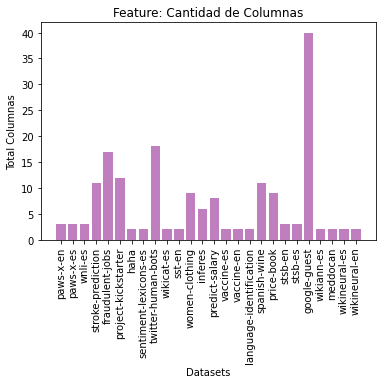
\includegraphics[width=\textwidth]{Graphics/results/columns.png}
          \caption{Columnas}
          \label{fig:columns}
    \end{minipage}      
    \hspace{0.02cm}
    \begin{minipage}[b]{0.5\textwidth}
      
        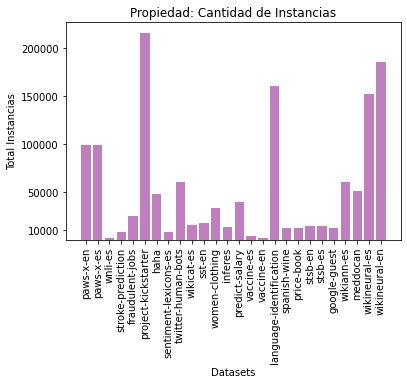
\includegraphics[width=\textwidth]{Graphics/results/instances.png}
          \caption{Instancias}
          \label{fig:instances}
        \end{minipage} 
\end{figure}

\begin{figure}[!h]
    \begin{minipage}[b]{0.5\textwidth}
        \centering
        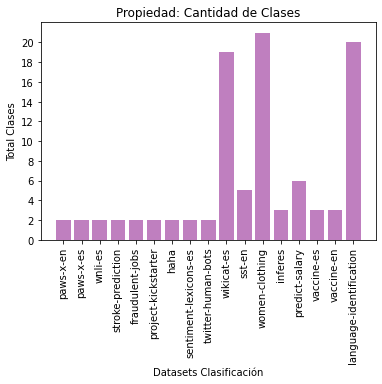
\includegraphics[width=\textwidth]{Graphics/results/class.png}
          \caption{Clases}
          \label{fig:clases}
    \end{minipage}      
    \hspace{0.02cm}
    \begin{minipage}[b]{0.5\textwidth}
        \centering
        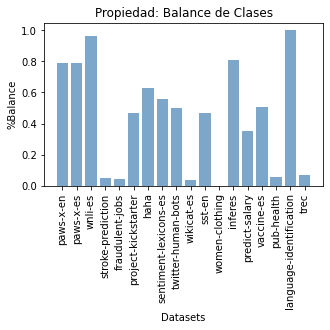
\includegraphics[width=\textwidth]{Graphics/results/balance.png}
          \caption{Balance de Clases}
          \label{fig:balance}
        \end{minipage} 
\end{figure}


\begin{figure}[!tbp]
    \centering
    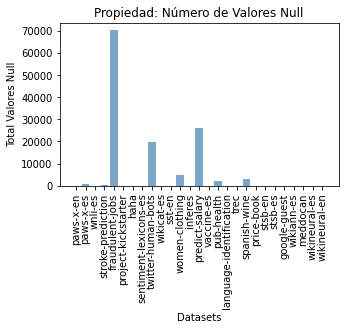
\includegraphics[width= 0.6\textwidth]{Graphics/results/null_values.png}
        \caption{Valores Null}
        \label{fig:null}
\end{figure}

\section{Sistemas AutoML}\label{section:AutoML}

En los ultimos años se han desarrollado una gran cantidad de marcos de aprendizaje automático, ya sea mediante la mejora iterativa de diseños antiguos o mediante 
el uso de enfoques novedosos. Estos se clasifican atendiendo a sus características internas y externas [\cite{52}]. Las características internas definen su 
funcionamiento, tales como el tipo y la variedad de algoritmos sobre los cuales realizan la búsqueda(características del espacio de búsqueda). Las externas 
destacan la utilidad de los sistemas. En esta categoría se encuentran los dominios a los que son aplicables. También las tareas que resuelven, ya sean las clásicas de 
aprendizaje automático o las específicas de dominios: relacionadas a imágenes, textos y series temporales. 

La unión de las características internas y externas determinan cuan eficientes y rápidos son los sistemas, aún más importante determinan qué problemas de la 
vida real resuelven.
Los problemas que agrupa \textit{HAutoML-Bench} poseen una complejidad en su estructura debido a la naturaleza de sus datos. Además, 
requieren técnicas de sus dominios de aplicación para su resolución. Este benchmark va dirigido a sistemas AutoML que sean capaces de flexibilizar sus tipos de entrada 
y que contengan los algoritmos necesarios para atacar la mayor cantidad de tareas. 
Se propone realizar un estudio de herramientas de AutoML para identificar cuáles pueden evaluarse en \textit{HAutoML-Bench} solo atendiendo a sus características.
Aunque existe una gran cantidad de herramientas de AutoML, solo se analiza una selección entre todas las existentes.

%Auto-Weka
Auto-Weka[\cite{8}] es uno de los primeros sistemas en darse a conocer, utiliza la biblioteca de aprendizaje Weka y está implementado en el lenhuaje Java. 
Su estrategia de recorrido del Espacio de Búsqueda está encaminado a los algoritmos basados en optimizacion bayesiana. El mismo está formado por modelos de ML 
clásicos ya sean lineales, basados en árboles, ensambles y otras familias. Sus técnicas de preprocesamiento son deficientes y con respecto al dominio son nulas, 
lo limitan a enfrentarse solo a problemas tabulares.

%AutoSklear
Auto-Sklearn[\cite{9}] extiende la propuesta de Auto-Weka en mejoramientos de eficiencia y Robustez. Ambos incluyen como estrategia de búsqueda la optimización 
bayesiana. Una de sus diferencias radica en la biblioteca de algoritmos, ya que este se implementa sobre Scikit-Learn de Python y además incluye meta-aprendizaje. 
Las técnicas de preprocesamiento de Auto-Sklearn son superiores a las de Auto-Weka, aun así solo puede ser aplicable a problemas en donde sus datos tienen forma 
numérica y/o categórica. 

%TPO y RECIPE
El marco TPOT [\cite{65}] comparte las limitaciones mencionadas y al igual que Auto-Sklearn está implementado sobre Scikit-Learn, pero también incluye un algoritmo de 
la biblioteca XGBoost. Su mayor diferencia con los anteriores es su estrategia de Búsqueda, la cual se basa en programación evolutiva. 
El sistema RECIPE [\cite{64}] comparte las características anteriores con TPOT incluyendo sus limitaciones. Este también se encuentra restringido a problemas que se 
modelan con datos estructurados y con propiedades tabulares. Sin embargo, posee una desventaja respecto a los anteriores y es que solo es aplicable a problemas de 
clasificación, mientras que Auto-Weka, Auto-Sklearn y TPOT permiten adicionalmente regresión. Entre las ventajas de RECIPE se encuentra que al utilizar una 
gramática para organizar el conocimiento adquirido sobre las exitosas canalizaciones creadas, evita la generación de canalizaciones no válidas. Además de que el 
espacio de búsqueda es mayor con respecto a los anteriores.

Se puede observar que estos 4 sistemas como características comunes presentan que los datos de entrada deben contener solo características tabulares.
Los conjuntos del benchmark no evalúan esta cualidad de manera independiente de los demás dominios. Además, incluyen una variedad de tipos de tareas como 
reconocimiento de entidades, procesamiento del lenguaje natural que van más allá de una simple clasificación o regresión. Las tareas que modelan 
exigen técnicas del dominio al que pertenecen. Estas propiedades afirman que Auto-Weka, Auto-Sklearn, TPOT y RECIPE carecen de flexibilidad para 
su evaluación en todos los conjuntos de \textit{HAutoML-Bench}.

Los sistemas que solo utilizan redes neuronales para su modelado también son sistemas AutoML. Los más utilizados son Auto-Keras[\cite{13}] y Auto-Pytorch[\cite{21}], 
ambos se basan en la optimización bayesiana. 
AutoPytorch[\cite{21}] como su nombre lo indica, está implementado sobre el framework Pytorch. Este incluye redes neuronales y técnicas de ensamble. 
Las técnicas de preparación de características y del dominio que posee lo resalta del resto en su categoría de sistema AutoDL. Además de que puede ser aplicado a 
problemas de clasificación y regresión sin muchas modificaciones.

Auto-Keras[\cite{13}] se encuentra implementado sobre la biblioteca Keras. Este, al igual que AutoPytorch en sus respectivas evaluaciones de lanzamiento, 
se evaluaron en conjuntos de dominio imagen y tabular. A pesar de esto, en el bechmark no existen conjuntos que solamente respondan a esos tipos. 
Auto-Keras tiene componentes para tratar con el dominio texto y problemas multimodales, sobre AutoPytorch no hay indicios de que sea flexible 
ante estos. 
Auto-Keras dice poder enfrentarse a conjuntos de texto y multimodales y en sus ejemplos de uso solo se demuestra con conjuntos juguetes, los cuales carecen de 
semántica al estar transformados. En conclusión no existe evidencia de que el sistema pueda evaluarse en datasets en donde los datos se encuentran no estructurados. 

Por último dos sistemas que son relativamente nuevos y que incluyen ambos enfoques: modelos de machine learning clásico y redes neuronales. 
Estos sistemas son AutoGOAL y AutoGluon.

AutoGOAL[\cite{40},\cite{41}] es una propuesta de AutoML heterogéneo que construye un espacio de búsqueda jerárquico mediante gramáticas libres del contexto y 
probabilidades. A diferencia de los anteriores sistemas, posee un proceso 
de introspección de código que se encarga de explorar sus bibliotecas base en búsqueda de algoritmos, en vez de utilizar implementaciones directas de las mismas.
Sus bibliotecas base son Scikit-learn, Nltk, Keras, Gensim y Pytorch.
Resuelve tareas clásicas de machine learning como clasificación, regresión y clustering. Además, problemas relacionados con dominios específicos como procesamiento 
del lenguaje natural. También resuelve tareas con imágenes y tabulares puros, como un extra permite resolver problemas de reconocimiento de entidades y relaciones.
Su implementación de tipos semánticos para la declaración de la entrada y salida de los problemas le permite utilizar datos estructurados y no estructurados. Sus 
tipos y la forma en que construye y recorre el espacio de búsqueda es lo que le permite resolver el problema de AutoML Heterogéneo. 
Existe evidencia de que AutoGOAL puede evaluarse en conjuntos de datos que contienen una y más columnas de texto. Sin embargo, en conjuntos de datos multimodales 
carecen de un tipo definido que permita modelar estas entradas.   

AutoGluon[\cite{17},\cite{42}]
%······················pending········································

\begin{table}[H]
  \centering
  \resizebox{10cm}{!} {
  \begin{tabular}{|l|c|c|c|c|c|}
  \hline
  Dataset & \multicolumn{3}{c|}{Texto} & \multicolumn{2}{c|}{Multimodales}\\ \hline
                        & Clasif   & Regres   & Entidades& Clasif   & Regres   \\ \hline
  Auto-Weka             &          &          &          &          &          \\
  Auto-Sklearn          &          &          &          &          &          \\
  TPOT                  &          &          &          &          &          \\ 
  RECIPE                &          &          &          &          &          \\
  AutoPytorch           &          &          &          &          &          \\
  Auto-Keras            &          &          &          &          &          \\
  AutoGOAL              &\checkmark&\checkmark&\checkmark&          &          \\
  AutoGluon             &\checkmark&\checkmark&          &\checkmark&\checkmark\\ \hline
                        &  10      &  2       &  4       &   8      &  3       \\ \hline
  \end{tabular}
  \caption{Evaluación Cualitativa de los sistemas sobre los conjuntos de datos del benchmark}
  \label{fig:eval-cuali}
  }
\end{table}


\section{Configuración Experimental}\label{section:seetings}
Las evidencias presentadas en el apartado \ref{section:AutoML} permiten concluir que tanto AutoGOAL como AutoGluon atendiendo a sus característica pueden evaluarse en 
algunos conjuntos del benchmark.
Para la evaluación cuantitativa AutoGluon es el sistema seleccionado. Este posee inicialmente la mayor cantidad de tareas que pudiera resolver con un total de 23. 
Además existen limitantes de tiempo y software que impiden la evaluación de ambos sistemas. 
En las próximas subsecciones se explica todo el marco experimental cuantitativo que pone a prueba el rendimiento de AutoGluon.

\subsection{Hadware}\label{subsection:hadware}
El hadware de evaluación seleccionado es la plataforma Colab. Esta cuenta con un entorno de ejecución en la nube que provee recursos para ejecutar programas 
escritos en el lenguaje Python. Los recursos presentes en la evaluación son: CPU de 12 GB de RAM máximo, 120 GB de almacenamiento de disco duro y 188 unidades de GPU.

\subsection{Configuración de los Sistemas AutoML}\label{subsection:conf-marcos}
AutoGluon se utiliza en su versión estable v0.5.2. Esta herramienta tiene muchos parámetros configurables en cada uno de sus modelos, tabular, multimodal, imagen y texto. 
Estos presentan su configuración predeterminada, exceptuando los que se describen a continuación.
\begin{itemize}
    \item Restricciones de software: AutoGluon se instala con GPU en vista a verificar su rápidez y rendimiento durante las pruebas. No existen limitaciones de RAM salvo
    las inpuestas por el entorno de ejecución.
    \item Métrica de optimización: Se utilizan para clasificación binaria: F1, clasificación multiclase: accuracy y para regresión el error cudrático medio. Todas se 
    ecuentran dentro de las métricas medidas en la evaluación.
    \item Restricciones de tiempo: selección de dos instantes de tiempo para la realización de las evaluaciones 5 min y 15 min. 
    \item Tamaño del conjunto de validación: utilizar un tamaño 0.2 del total de instancias que equivale a un 20\%. 
    \item Parámetros obligatorios: la etiqueta de la columna salida.  
\end{itemize}
\section{Resultados}\label{section:results}
La experimentación cuantitativa incluye tres evaluaciones de AutoGluon sobre todos los conjuntos de datos.
La primera ronda de ejecuciones tiene como objetivo medir el rendimiento de AutoGluon durante 5 minutos de entrenamiento por conjunto. Sus parámetros 
se encuentran en sus valores por defecto, solo se especifican los mencionados anteriormente \ref{subsection:conf-marcos}. 

La segunda ronda pretende obtener resultados aumentado la cantidad de tiempo a 15 minutos de entrenamiento por conjunto. Se mantienen los mismos parámetros por defecto.

Estas primeras ejecuciones tienen como meta evaluar al sistema realizando su propia inferencia de tipos en intento de mitigar la ayuda externa hacia el sistema. Además 
se quiere ver si la herramienta es sencible a los cambios de tiempo, posibilitando alguna mejora en todos los conjuntos.

En la última ronda se quiere ver si al introducir el tipo semántico de cada columna, AutoGluon mantiene su consistencia en los resultados. 

En las figuras se muestran los valores obtenidos durante la evaluación, se encuentran separados en los diferentes tipos de tareas. Las métricas que se muestran
para cada tareas son la utilizada para la optimización y la métrica ideal propuesta en el apartado \ref{subsection:metrics}. 
Recordar que para la clasificación es \textit{balanced-accuracy} y para regresión \textit{RMSE}.

\subsection{Errores de los sistemas durante el marco experimental}\label{subsection:errors}
AutoGluon presenta fallas durante las ejecuciones de algunos conjuntos. Estos para poder evaluarse tienen que ser sometidos a transformaciones.

El dataset women-clothing contiene una clase que solo posee una intancia. También posee valores faltantes en su columna salida. En ambos casos AutoGluon se 
limita a resolver problemas de este tipo. Para que el sistema pueda ejecutarse las instancias con problemas son removidas.

El conjunto google-guest tiene en su etiqueta final un número de valores distintos bastante pequeño. En su definición original este modela una tarea de regresión, en 
donde los valores de la etiqueta final pueden estar en el rango [0,1]. AutoGluon infiere incorrectamente el tipo de tarea, lo que produce errores en la ejecución, para 
dar una solución se introduce el tipo de tarea solamente para este conjunto.

Estas ejecuciones fallidas ocurren durante la primera ronda de pruebas. Las soluciones a estos problemas deben ser utilizadas en las restantes rondas. 
En la última ocurren errores al introducir los tipos semánticos de cada una de las columnas. Las primeras limitaciones se dan al no poder introducir como 
parámetro de entrada el tipo datetime, que hace referencia a los tipos de tiempo y fecha. Además, en el procesamiento del tipo path\_image de AutoGluon si este no 
coincide con el directorio o un archivo tipo imagen, el sistema reporta errores. Ambos tipos fueron apartados de la entrada. 
El conjunto spanish-wine en sus entradas etiquetadas como numéricas y que presentan datos faltantes AutoGluon detiene la ejecución. Al ser pocas instancias se remueven.

\begin{table}[H]
  \centering
  \resizebox{15cm}{!} {
  \begin{tabular}{|l|cccccc|}
  \hline
          & \multicolumn{4}{p{8cm}|}{Tiempo: 5 min}  & \multicolumn{2}{p{4cm}|}{Tiempo: 15 min}\\  \hline
          & \multicolumn{2}{p{4cm}|}{Valores por defecto} & \multicolumn{2}{p{4cm}|}{Entradad de Tipo} & \multicolumn{2}{p{4cm}|}{Valores por defecto}\\ \hline
  Dataset & F1 & bala-acc & F1  & bal-acc & F1 & bal-acc  \\ \hline
  paws-x-en             & 0.931 & 0.940 & 0.917 & 0.928 & 0.947 & 0.953 \\
  paws-x-es             & 0.840 & 0.856 & 0.837 & 0.852 & 0.875 & 0.888 \\
  wnli-es               & 0.61  & 0.5   & 0.613 & 0.5   & 0.613 & 0.5   \\ 
  stroke-prediction     & 0.0   & 0.5   & 0.0   & 0.5   & 0.0   & 0.5 \\
  fraudulent-jobs       & 0.0   & 0.5   & 0.0   & 0.5   & 0.732 & 0.818 \\
  project-kickstarter   & 0.074 & 0.498 & 0.225 & 0.499 & 0.153 & 0.502 \\
  haha                  & 0.764 & 0.807 & 0.761 & 0.803 & 0.774 & 0.814 \\
  sentiment-lexicons-es & 0.747 & 0.770 & 0.747 & 0.770 & 0.775 & 0.794 \\ 
  twitter-human-bots    & 0.680 & 0.770 & 0.676 & 0.759 & 0.721 & 0.791 \\ \hline

  \end{tabular}
  \caption{Resultados en tareas de Clasificación Binaria}
  \label{fig:class-binary}
  }
\end{table}

\begin{table}[H]
  \centering
  \resizebox{15cm}{!} {
  \begin{tabular}{|l|cccccc|}
  \hline
          & \multicolumn{4}{p{8cm}|}{Tiempo: 5 min}  & \multicolumn{2}{p{4cm}|}{Tiempo: 15 min}\\  \hline
          & \multicolumn{2}{p{4cm}|}{Valores por defecto} & \multicolumn{2}{p{4cm}|}{Entradad de Tipo} & \multicolumn{2}{p{4cm}|}{Valores por defecto}\\ \hline
  Dataset & acc & bala-acc & acc  & bal-acc & acc & bal-acc  \\ \hline
  wikicat-es              & 0.385 & 0.268 & 0.385 & 0.268 & 0.603 & 0.518 \\
  sst-en                  & 0.580 & 0.549 & 0.580 & 0.549 & 0.577 & 0.545 \\
  women-clothing          & 0.671 & 0.449 & 0.677 & 0.456 & 0.760 & 0.642 \\ 
  inferes                 & 0.691 & 0.680 & 0.651 & 0.647 & 0.767 & 0.759 \\
  predict-salary          & 0.199 & 0.178 & 0.190 & 0.173 & 0.191 & 0.172 \\
  language-identification & 0.966 & 0.966 & 0.966 & 0.966 & 0.976 & 0.976 \\
  vaccine-es              & 0.780 & 0.756 & 0.779 & 0.743 & 0.779 & 0.766 \\
  pub-health              & 0.609 & 0.370 & 0.609 & 0.370 & 0.759 & 0.576 \\ 
  trec                    & 0.962 & 0.912 & 0.966 & 0.933 & 0.970 & 0.972 \\ \hline

  \end{tabular}
  \caption{Resultados en tareas de Clasificación Multiclase}
  \label{fig:class-multi}
  }
\end{table}

\begin{table}[H]
  \centering
  \resizebox{15cm}{!} {
  \begin{tabular}{|l|c|c|c|}
  \hline
  Dataset & 5 min sin inferencia  & 5min con Inferencia & 15min con Inferencia \\ \hline
               & RMSE   & RMSE  & RMSE  \\ \hline
  spanish-wine & 13.8   & 14.709 & Image  \\
  stsb-en      & 0.72   & 0.693  & Image  \\
  stsb-es      & 0.955  & 0.955  & Image  \\ 
  price-book   & 596.9  & 477.47 &  Image  \\
  google-guest & 0.443  & 0.50   &  Image  \\ \hline

\end{tabular}
  \caption{Regresión}
  \label{fig:regression}
  }
\end{table}

\section{Discusiones}\label{section:discussions}
AutoGluon con respecto a sus méricas
de optimización es bastante restrictivo, se intentó cambiar de métricas en ciertos modelos y no se obtuvo buenos resultados. A pesar de ello las métricas esco